% --------------------------------------------------------------------------------
\newpage
\section{Auditory Peripheral Module}
% --------------------------------------------------------------------------------

% Make general target
\hypertarget{Concepts:AuditoryPeripheralModule}{}

% Make target for following functions:
\hypertarget{Concepts:IPEMCalcANI}{}
\hypertarget{Concepts:IPEMCalcANIFromFile}{}
\hypertarget{Concepts:IPEMLoadANI}{}
\hypertarget{Concepts:IPEMSaveANI}{}

\subsection{Introductory description}
% --------------------------------------------------------------------------------

The Auditory Peripheral Module (APM) (fig. \ref{Fig:ModulesAPM})
takes as input a sound and gives as output the \emph{auditory
primary image} which is a kind of physiological justified
representation of the auditory information stream along the VIIIth
cranial nerve. The musical signal is decomposed in different
subbands and represented as neural patterns. The patterns are
rate-codes, which means that they provide the probability of
neuronal firing during a short interval of time.
\begin{figure}[h]
    \centering
    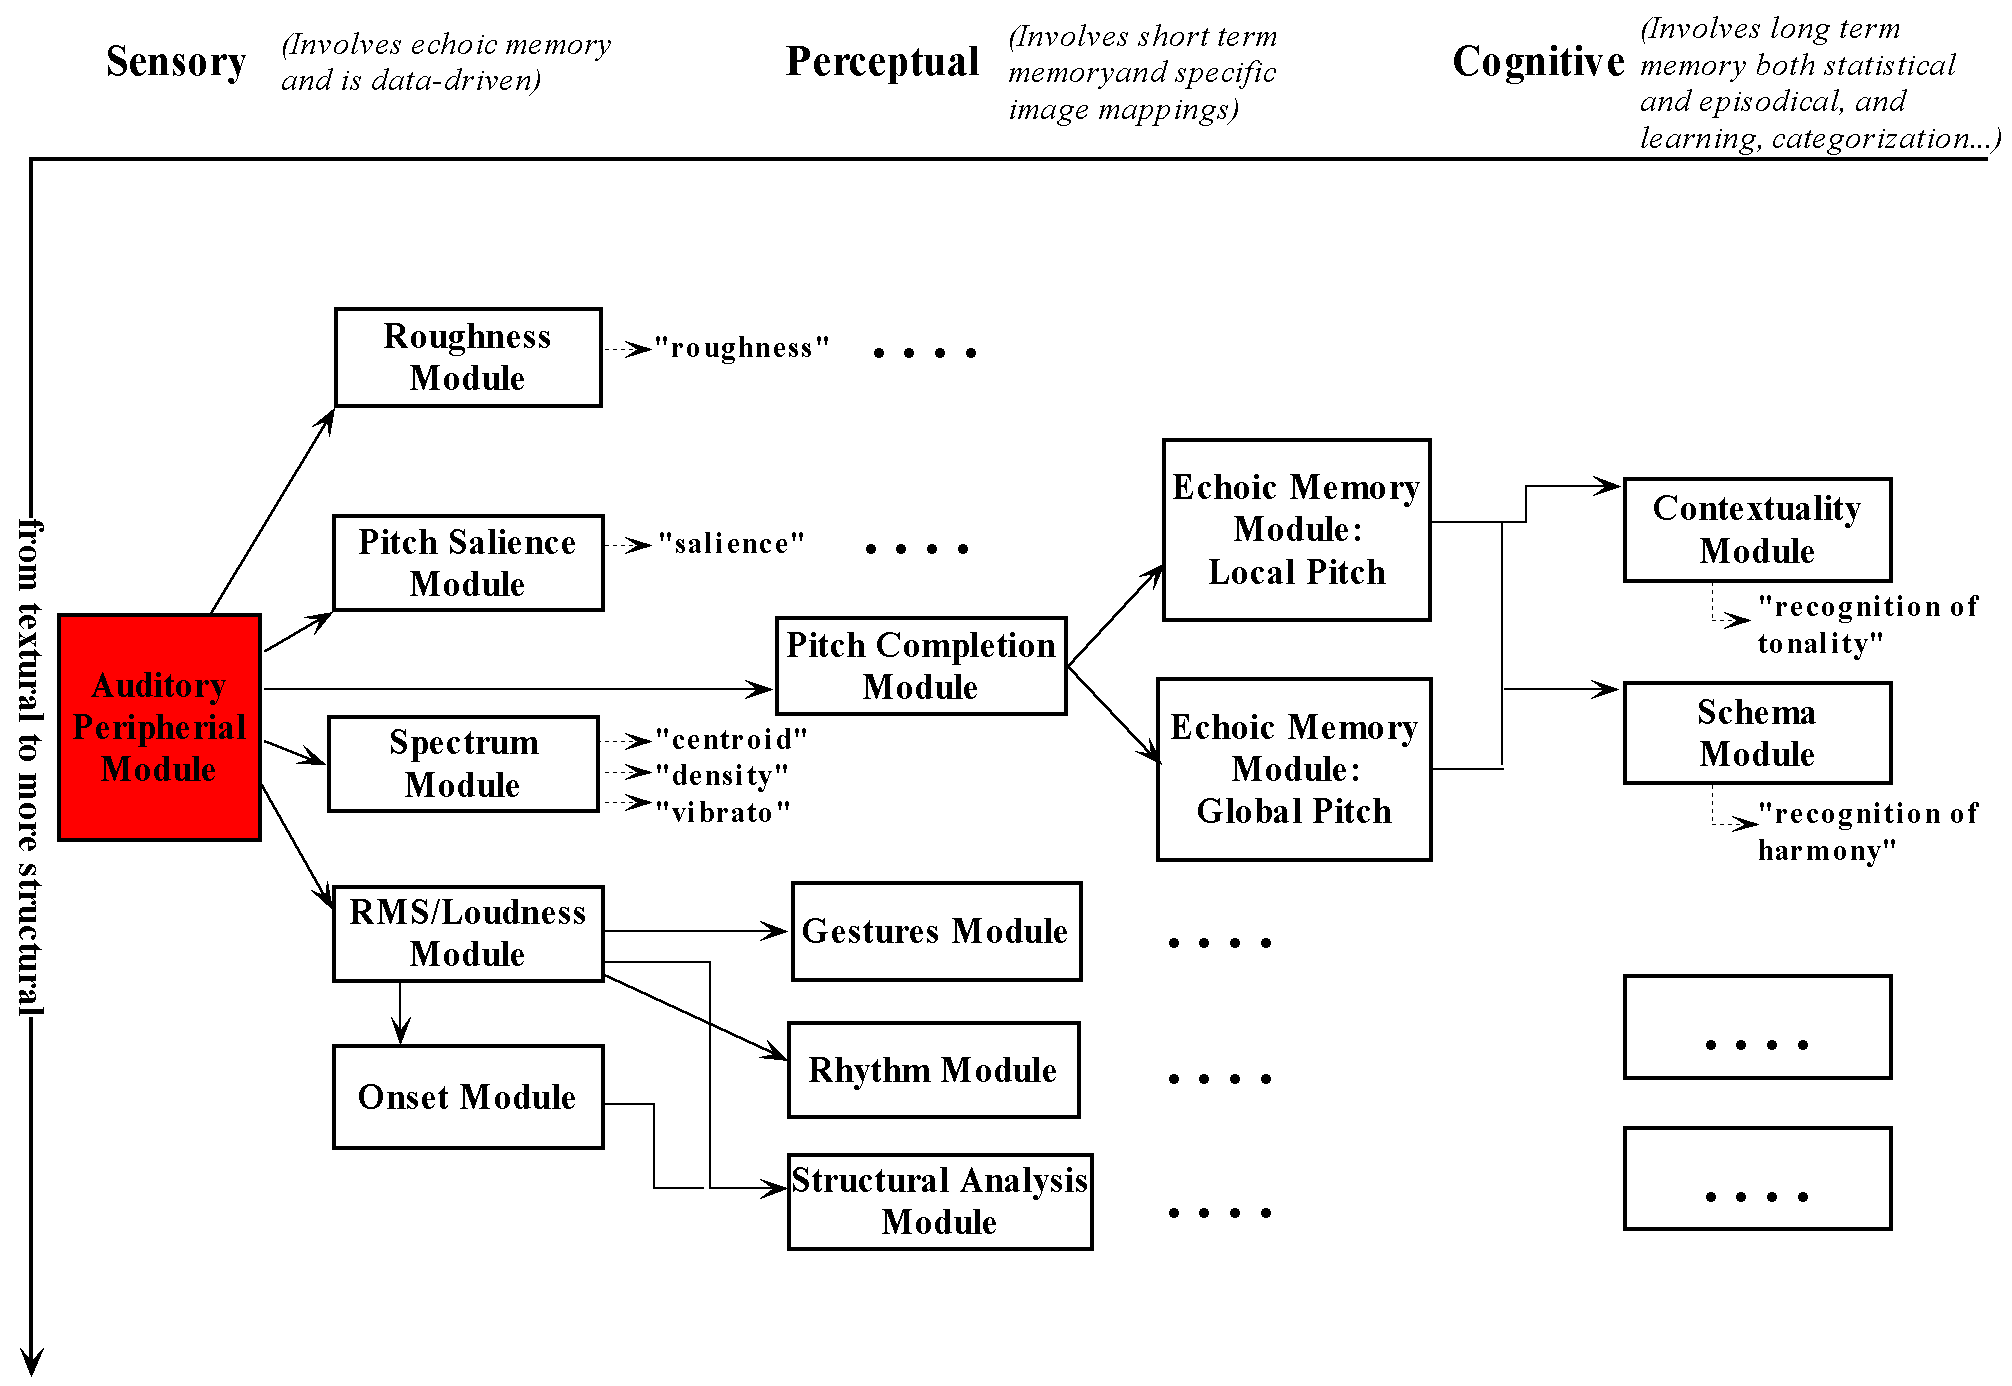
\includegraphics[width=\textwidth]{Graphics/ModulesAPM}
    \caption{Chart of image transformation modules, with APM highlighted}
    \label{Fig:ModulesAPM}
\end{figure}

The Auditory Peripheral Module that we use is an adapted version
of \citeA{VanImmerseelMartens:92} model of the auditory periphery.
The processing stages involve:
\begin{itemize}
\item
    Simulation of the filtering of the outer and middle ear.
\item
    Simulation of basilar membrane resonance in the inner ear. This is
    implemented by an array of band-pass filters whose center
    frequencies are spaced on a critical band scale (Bark scale).
    The bandwidth of each filter equals
    a critical band.
\item
    Simulation of a hair cell model. This converts the band-pass filtered signals into
    neural {\sl rate-code} patterns. This operation deals with half-wave rectification and
    dynamic range compression.
\end{itemize}

Figure \ref{Fig:APMModule} gives a view of the transformation of
sound into primary images.
\begin{figure}[h]
    \centering
    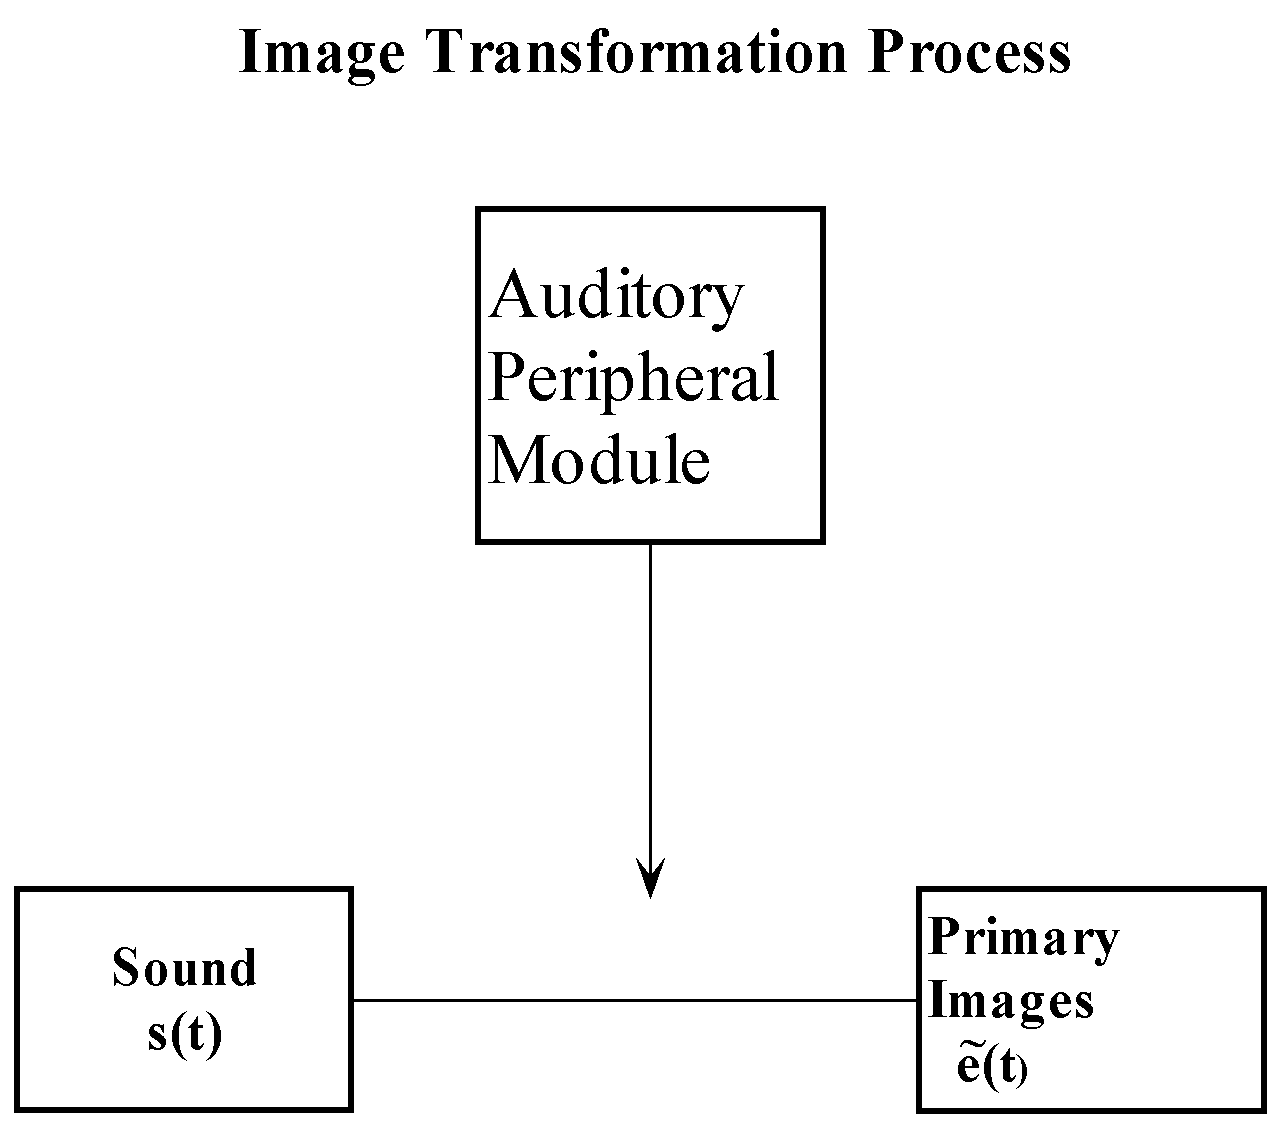
\includegraphics[width=\IPEMDefaultFigureWidth]{Graphics/APMModule}
    \caption{Image Transformation Process: Auditory Peripheral  Module}
    \label{Fig:APMModule}
\end{figure}

\subsection{Functional-logical description}
% --------------------------------------------------------------------------------

The APM can be described as a function which transforms a musical
sound signal $s(t)$ into a set of patterns $e_n(t)$ (with $n = 1,
2, ..., C$) that encode the responses of auditory neuronal fibers
spread along the basilar membrane (see Equation \ref{Eq1}). The
auditory filters, sometimes also called {\sl channels}, simulate
the neuronal band-pass characteristics and the firing rate
encoding. The frequency range covered by the auditory filters
depends on the center frequencies of the filters, the number of
chosen channels and the chosen distance between the channels. In
most of our simulations we chose forty channels ($C=40$), half a
critical band apart from each other. This covers a range from 140
Hz to 8877 Hz. As a short-hand we use the notation:

\begin{displaymath}
APM:~s(t) \rightarrow \left[
\begin{array}{l}
e_1(t) \\ e_2(t) \\ \cdots \\ e_{C}(t)
\end{array}
\right]=~e(t,c)~=~\tilde{e}(t)
\end{displaymath}
or, alternatively,
\begin{equation}
APM:~s(t) \rightarrow \tilde{e}(t) \label{Eq1}
\end{equation}

The pattern denoted $\tilde{e}(t)$ is called the \emph{primary
image} or \emph{auditory nerve image (ANI)} of $s(t)$. It should
be considered the auditory counterpart of D.~Marr's {\sl primal
sketch} in the domain of visual perception \cite{Marr:82}. The
tilde character here denotes a vector in which each
vector-component corresponds to one auditory filter. The arrow
represents a causal transformation, in this case from a sound into
the auditory nerve image.

In our terminology, a \emph{running vector} means that the values
of the vector-components change over time, where $t$ denotes time.
The pattern $\tilde{e}(t)$ thus represents the neural activation
in all subbands over subsequent time steps. The notation $e(t,c)$
means the same, whereas $e(t,c)$ for fixed $c$ is the neural
activation in one particular channel $c$.

\subsection{Signal processing description}
% --------------------------------------------------------------------------------
For a full description of this module we refer to
\citeA{VanImmerseelMartens:92}. We limit ourselves to a more technical
verbal summary.

The auditory peripheral module simulates the cochlear mechanical
filtering using an array of overlapping band-pass filters.
%The
%module provides rate-code patterns of neural discharge at the
%level of the auditory nerve, representing the amount of neural
%excitation during short time intervals.
The basic steps of this model, shown in figure
\ref{Fig:AuditoryModel} can be summarized as follows.

\begin{figure}[h]
    \centering
    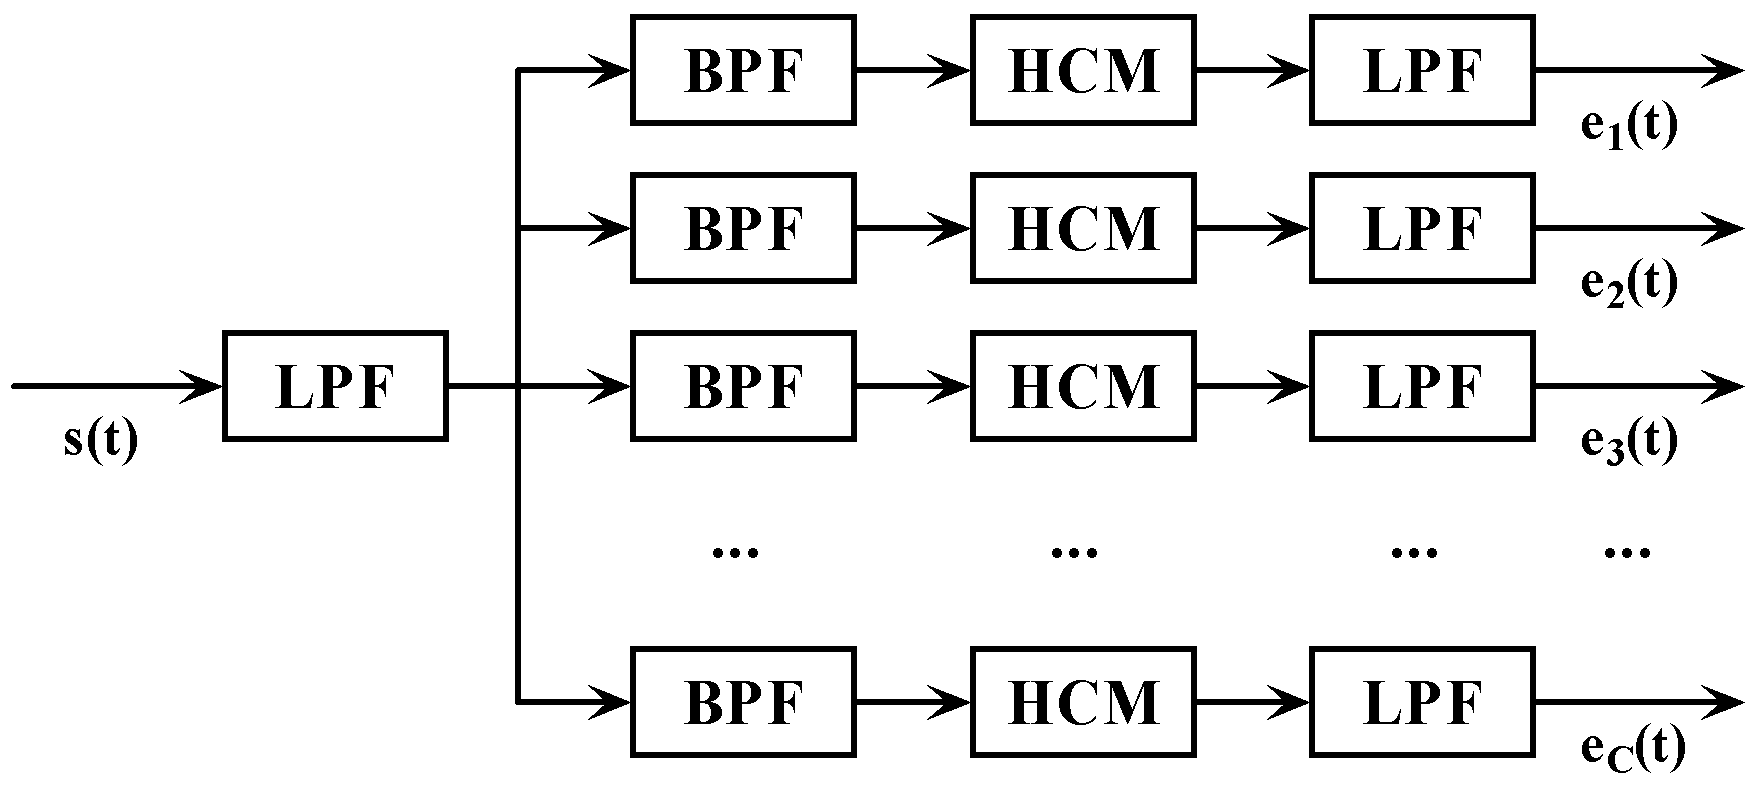
\includegraphics[width=\IPEMDefaultFigureWidth]{Graphics/AuditoryModel}
    \caption{Schema of the Auditory Peripheral Module. }
    \label{Fig:AuditoryModel}
\end{figure}

\begin{itemize}
\item
    The outer and inner ear filtering is implemented as a
    second-order low-pass filter (LPF) with a resonance frequency of
    4 kHz. This accounts for the overall frequency response of the
    ear, a coarse approximation to the Fletcher-Munson curves.
\item
    The filtering in the cochlea is implemented by an array of
    band-pass filters (BPF). In many of the simulations in this book,
    we use center frequencies that are spaced equidistantly on a
    critical band scale, having an overlap of half a critical band.
    Forty channels are used with center frequencies ranging from 141
    to 8877 Hz. The filters have a 3 dB bandwidth of one critical
    band; a low-frequency slope of about 10 dB per critical band unit
    and a high-frequency slope of about 20 dB per critical band unit.
\item
    The mechanical to neural transduction is performed by a hair cell
    model (HCM), which is assumed identical in all channels. The HCM
    is a forward-driven gain controlled amplifier that incorporates
    half-wave rectification and dynamic range compression. The HCM
    introduces distortion products that reinforce the low frequencies
    that correspond to the frequency of the beats.
\item
    A low-pass filter at 1250 Hz does an envelope extraction of the
    patterns in each channel. This low-pass filter accommodates for
    the loss of synchronization observed in the primary auditory
    nerve. The filter can be argued to have an effect on the width of
    the critical band for high $f_c$ although these may fall out of
    the scope of most musically relevant tones
    \cite{GreenwoodJoris:1996}.
\end{itemize}

The output $e(t,c)$ for fixed $c$ represents the rate-code of
neural discharge in channel $c$. This pattern is also called the
\emph{auditory nerve pattern} in channel $c$.

\subsection{Implementation}
% --------------------------------------------------------------------------------

\begin{tabularx}{\linewidth}{llX}
\hyperlink{FuncRef:IPEMCalcANI}{IPEMCalcANI} & - & Calculates auditory nerve image from signal\\
\hyperlink{FuncRef:IPEMCalcANIFromFile}{IPEMCalcANIFromFile} & - & Calculates auditory nerve image directly from sound file\\
\hyperlink{FuncRef:IPEMLoadANI}{IPEMLoadANI} & - & Loads auditory nerve image from .mat file\\
\hyperlink{FuncRef:IPEMSaveANI}{IPEMSaveANI} & - & Saves auditory nerve image to .mat file\\
\end{tabularx}

\subsection{Examples}
% --------------------------------------------------------------------------------

In this section we provide some examples of how to transform
musical signals into primary images (auditory nerve images). A
straightforward function is
\hyperlink{FuncRef:IPEMCalcANIFromFile}{IPEMCalcANIFromFile} which
allows you to read in a wav-file. If the wav-file
\emph{SchumannKurioseGeschichte.wav} is stored in the "Sounds"
subdirectory of the default input directory (see also the
\hyperlink{ReferenceManual:Installation}{installation}
instructions), and you agree with the default 40 subbands and the
overlap of 1/2 critical band, then the function is simply:\\

\IPEMCodeExtract{IPEMCalcANIFromFile('SchumannKurioseGeschichte.wav',[],[],1);}\\

Similarly, if \emph{ShepardCChord.wav} is stored in that same directory, you can write:\\

\IPEMCodeExtract{IPEMCalcANIFromFile('ShepardCChord.wav');}\\

The results should be similar to what you see on these pages
(except the score, of course):
\begin{enumerate}
\item
    Figure \ref{Fig:SchumannScore} shows the score of the
    \IPEMSound{Sounds/SchumannKurioseGeschichte.wav}{used
    excerpt of Schumann's Kuriose Geschichte}.
    \footnote{Robert Schumann "Kinderszenen-Kreisleriana", played
    by Martha Argerich (Deutsche Grammophon 410 653-2, 1984)}
\item
    Figure \ref{Fig:SchumannANIandAudioSignal} shows the results of processing
    this short excerpt with the Auditory Peripheral Module. The upper panel shows
    the waveform, the lower panel shows the primary image.
\item
    Figure \ref{Fig:ShepardCChordANIandAudioSignal} shows the results of processing
    \IPEMSound{Sounds/ShepardCChord.wav}{a signal consisting of
    the C major chord, build up from 3 Shepard tones} with the Auditory Peripheral Module.
    Again, the upper panel shows the waveform, the lower panel shows the primary image.
\end{enumerate}

To generate a Shepard-chord yourself, you can type (see
\hyperlink{FuncRef:IPEMShepardToneComplex}{IPEMShepardToneComplex}):\\

\IPEMCodeExtract{MyShepardChord = IPEMShepardToneComplex([1 0 0 0 1 0 0 1 0 0 0 0],1,22050,1);}\\

Now you generated a signal that is stored in
\IPEMCodeExtract{MyShepardChord}. And you can play it in the usual
MATLAB way with:\\

\IPEMCodeExtract{sound(MyShepardChord,22050);}\\

Pay attention to the fact that \IPEMCodeExtract{MyShepardChord} is
a signal in the MATLAB environment, not a wav-file. To process
this signal with the auditory peripheral module you can do:\\

\IPEMCodeExtract{IPEMCalcANI(MyShepardChord,22050);}\\

Note that the number 22050 is the sampling rate which should be
specified, and \IPEMCodeExtract{MyShepardChord} is a variable in
MATLAB, therefore it should not be between quotes.

\begin{figure}[h]
    \centering
    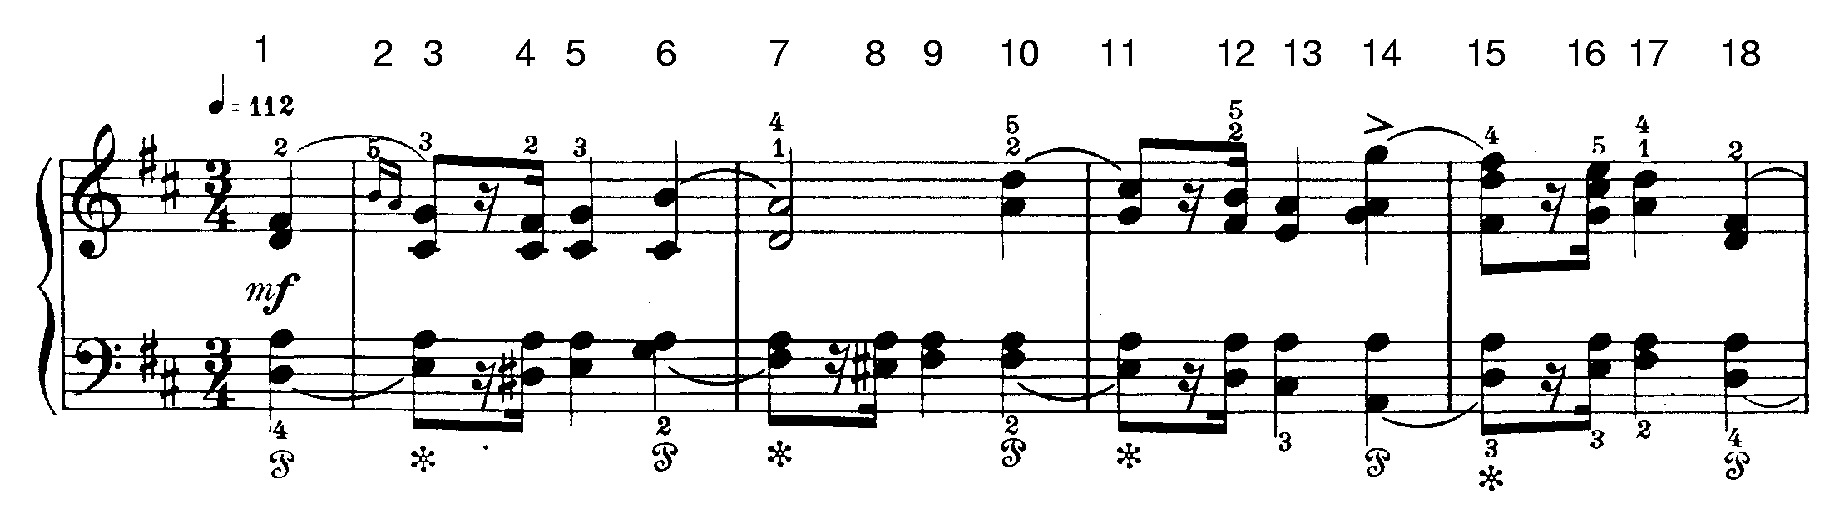
\includegraphics[width=\IPEMDefaultFigureWidth]{Graphics/SchumannScore}
    \caption{The first four measures of Schumann's piece "Kuriose Geschichte"}
    \label{Fig:SchumannScore}
\end{figure}

\begin{figure}[h]
    \centering
    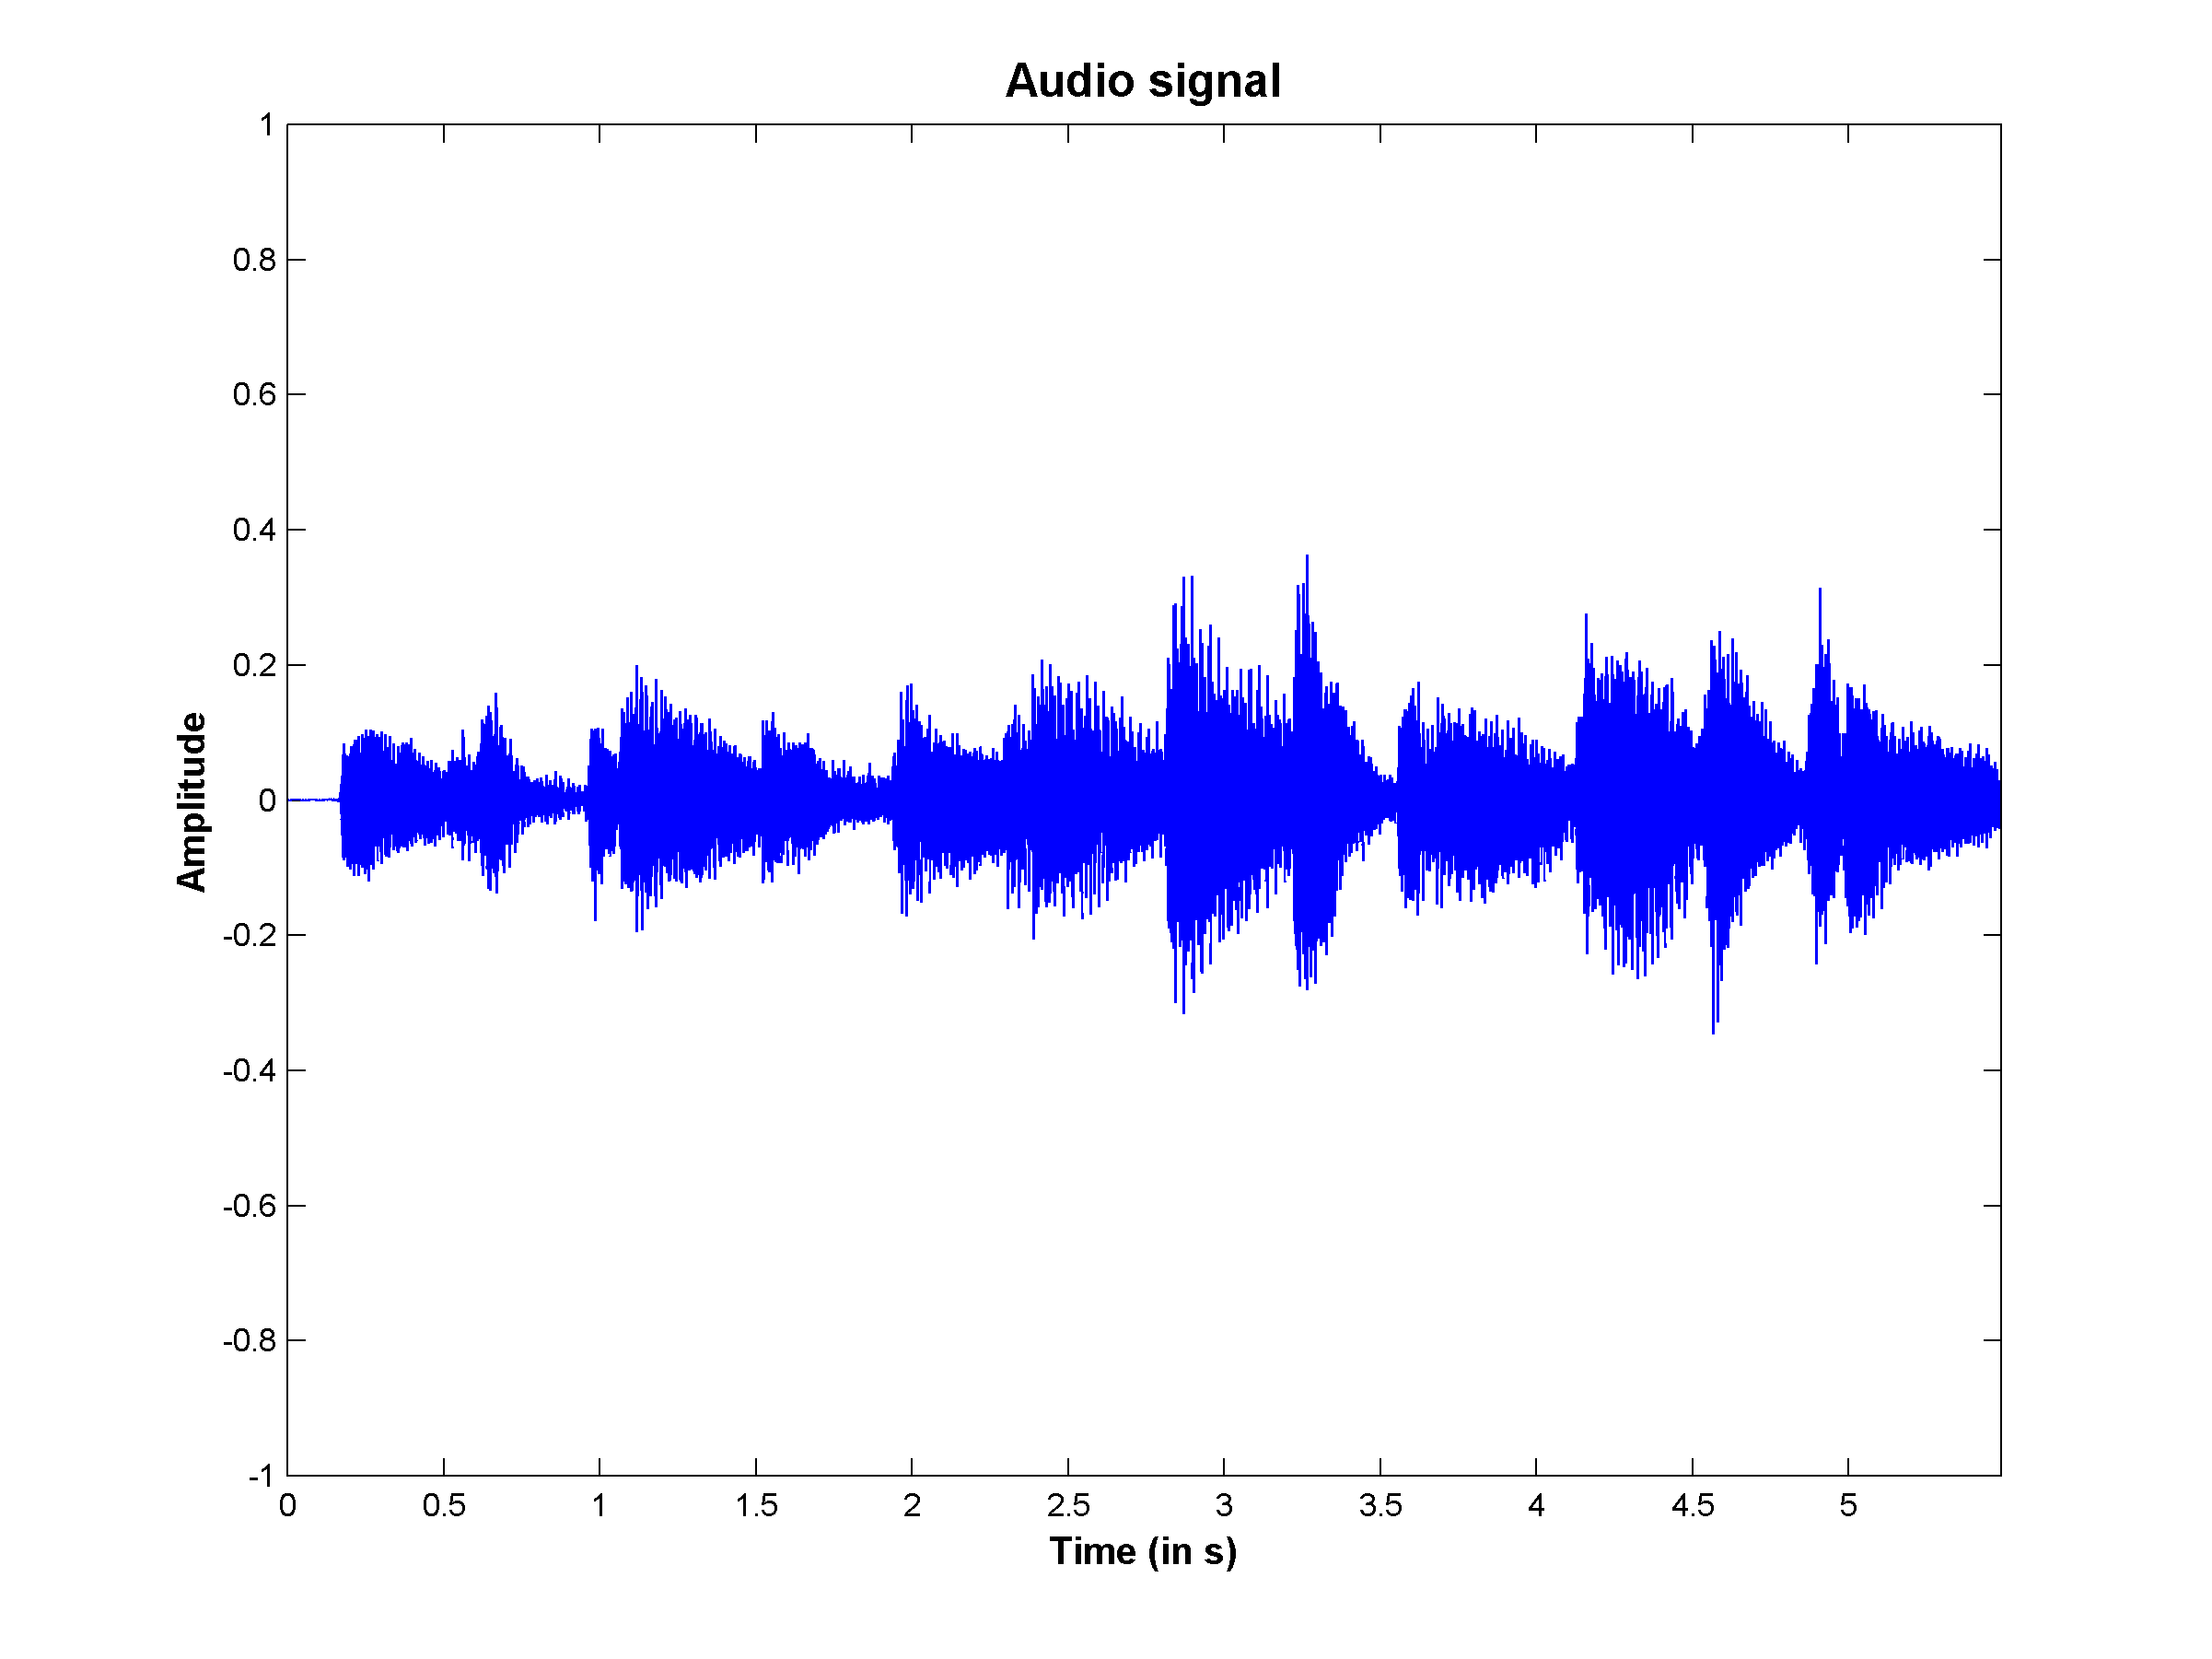
\includegraphics[width=\IPEMDefaultFigureWidth]{Graphics/SchumannAudioSignal}
    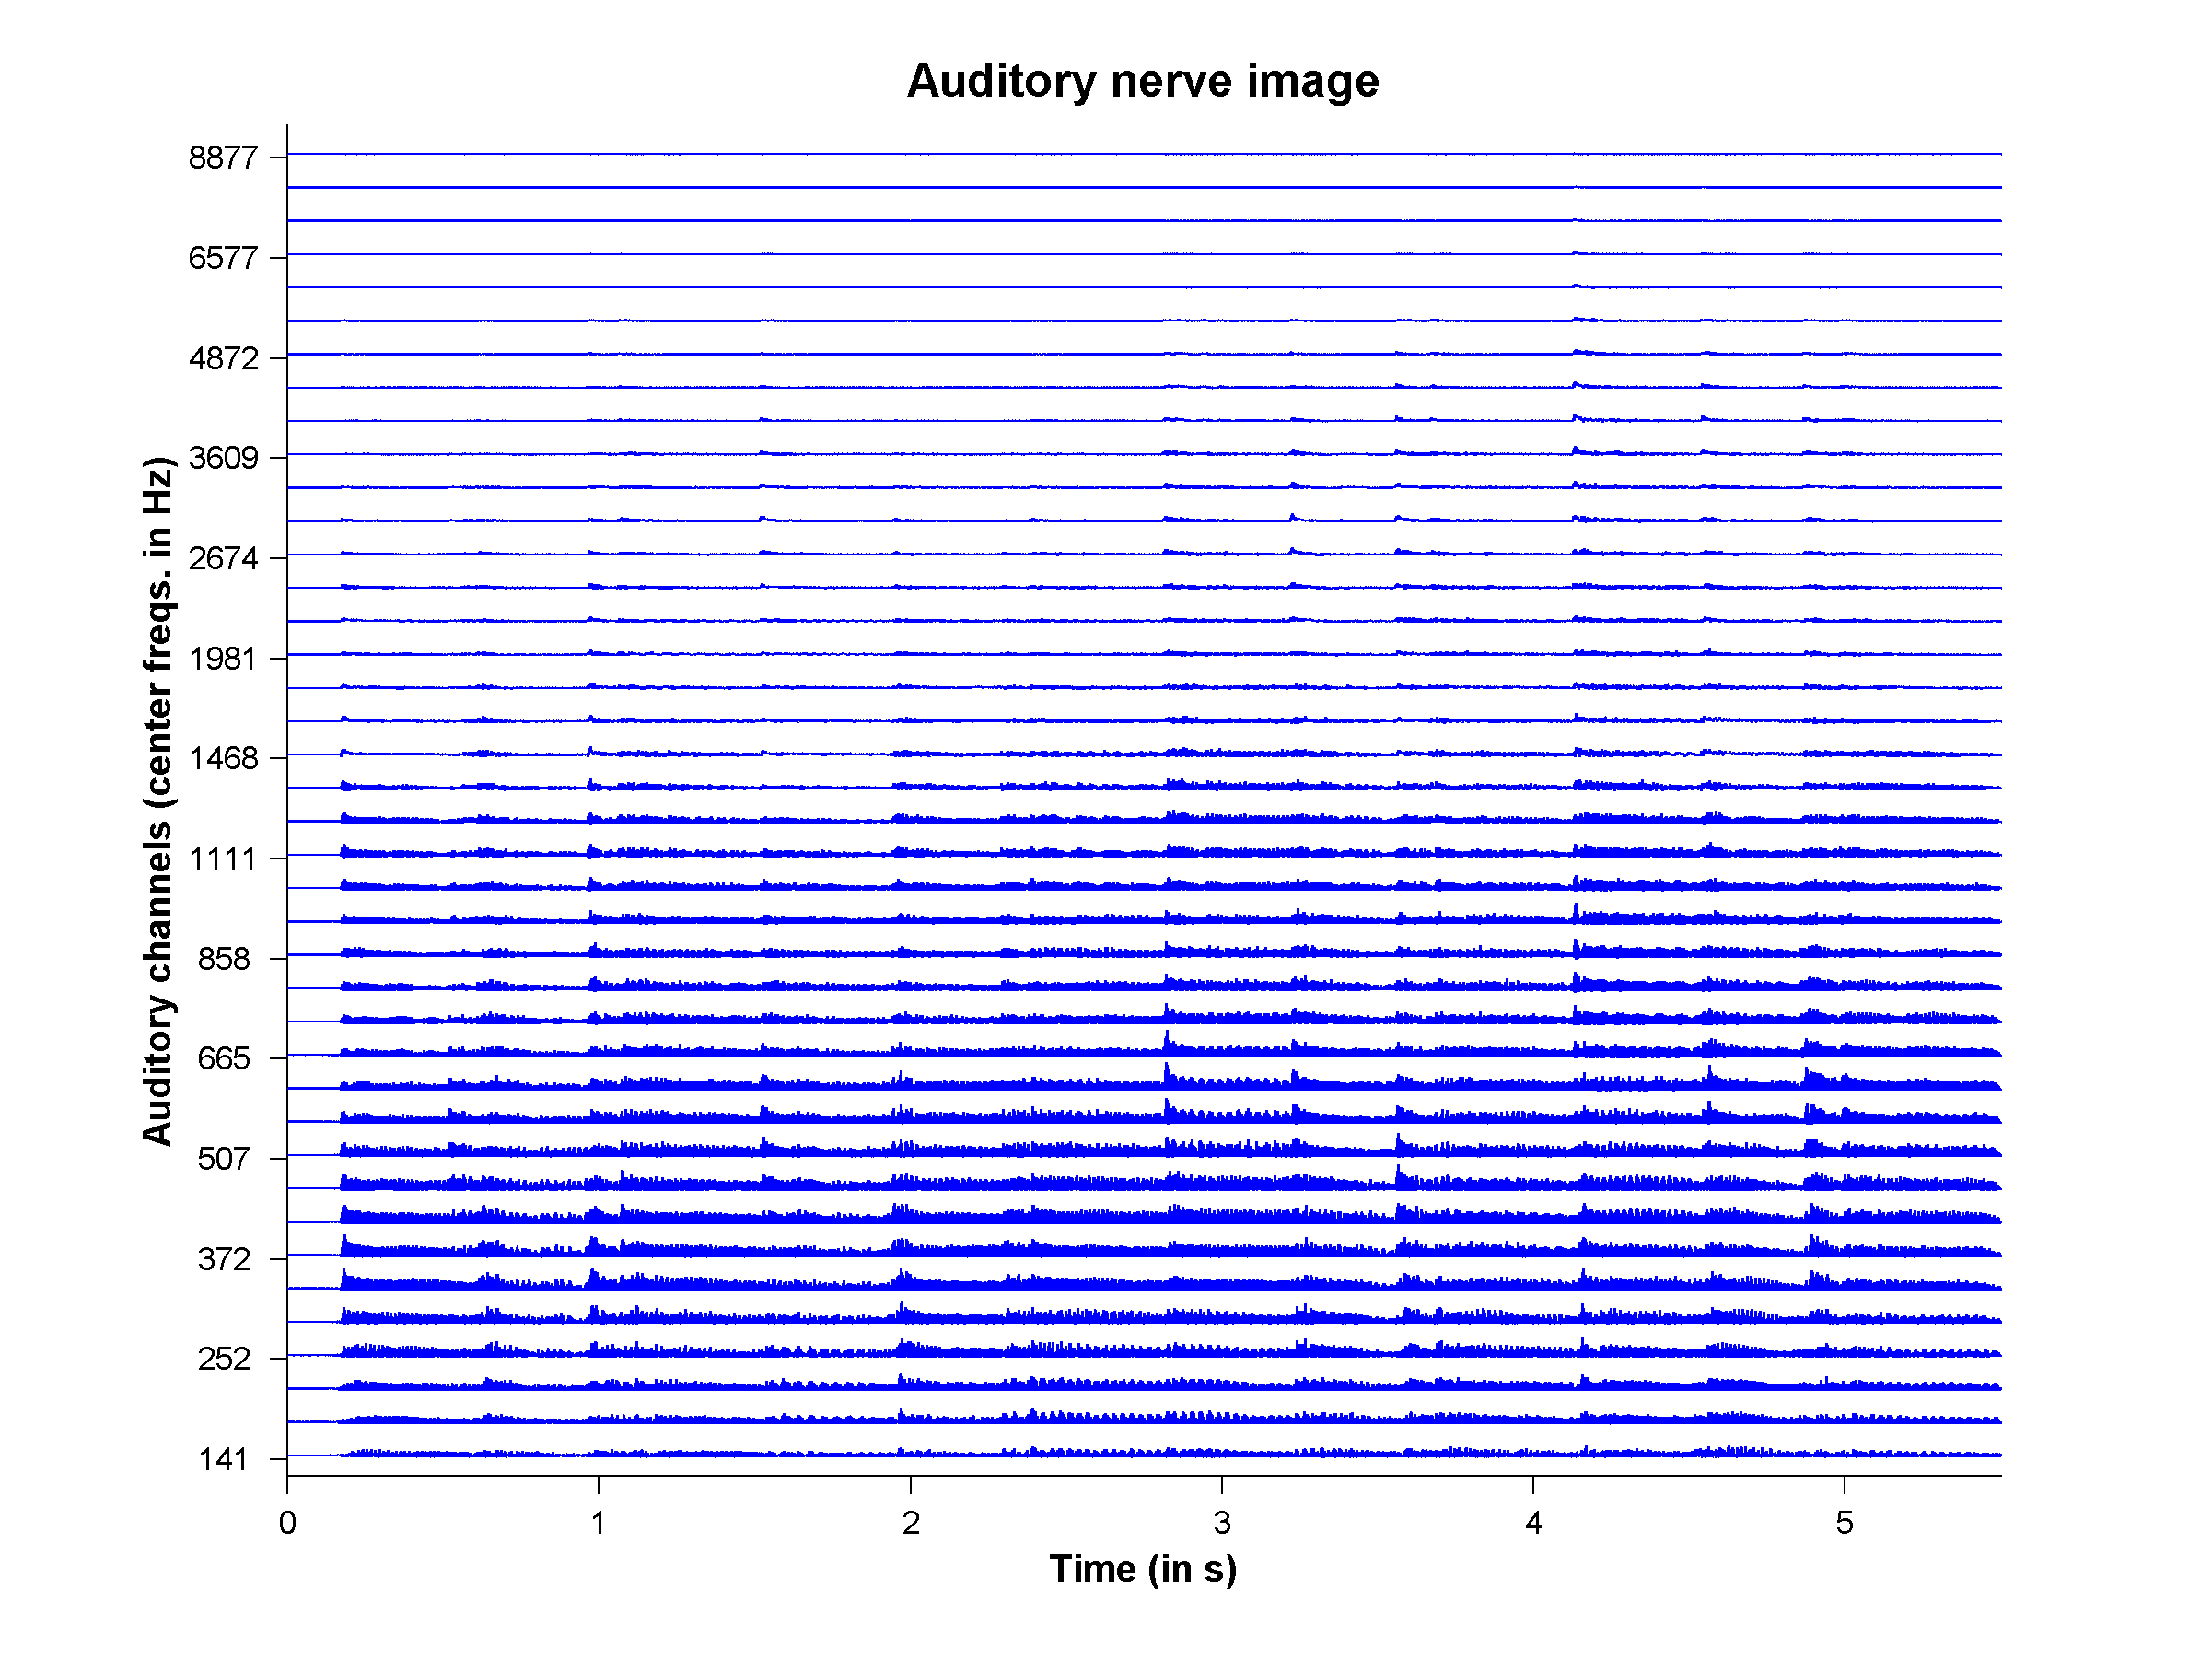
\includegraphics[width=\IPEMDefaultFigureWidth]{Graphics/SchumannANI}
    \caption{Top: waveform of a short excerpt of Schumann's Kuriose Geschichte. Bottom: primary image}
    \label{Fig:SchumannANIandAudioSignal}
\end{figure}

\begin{figure}[h]
    \centering
    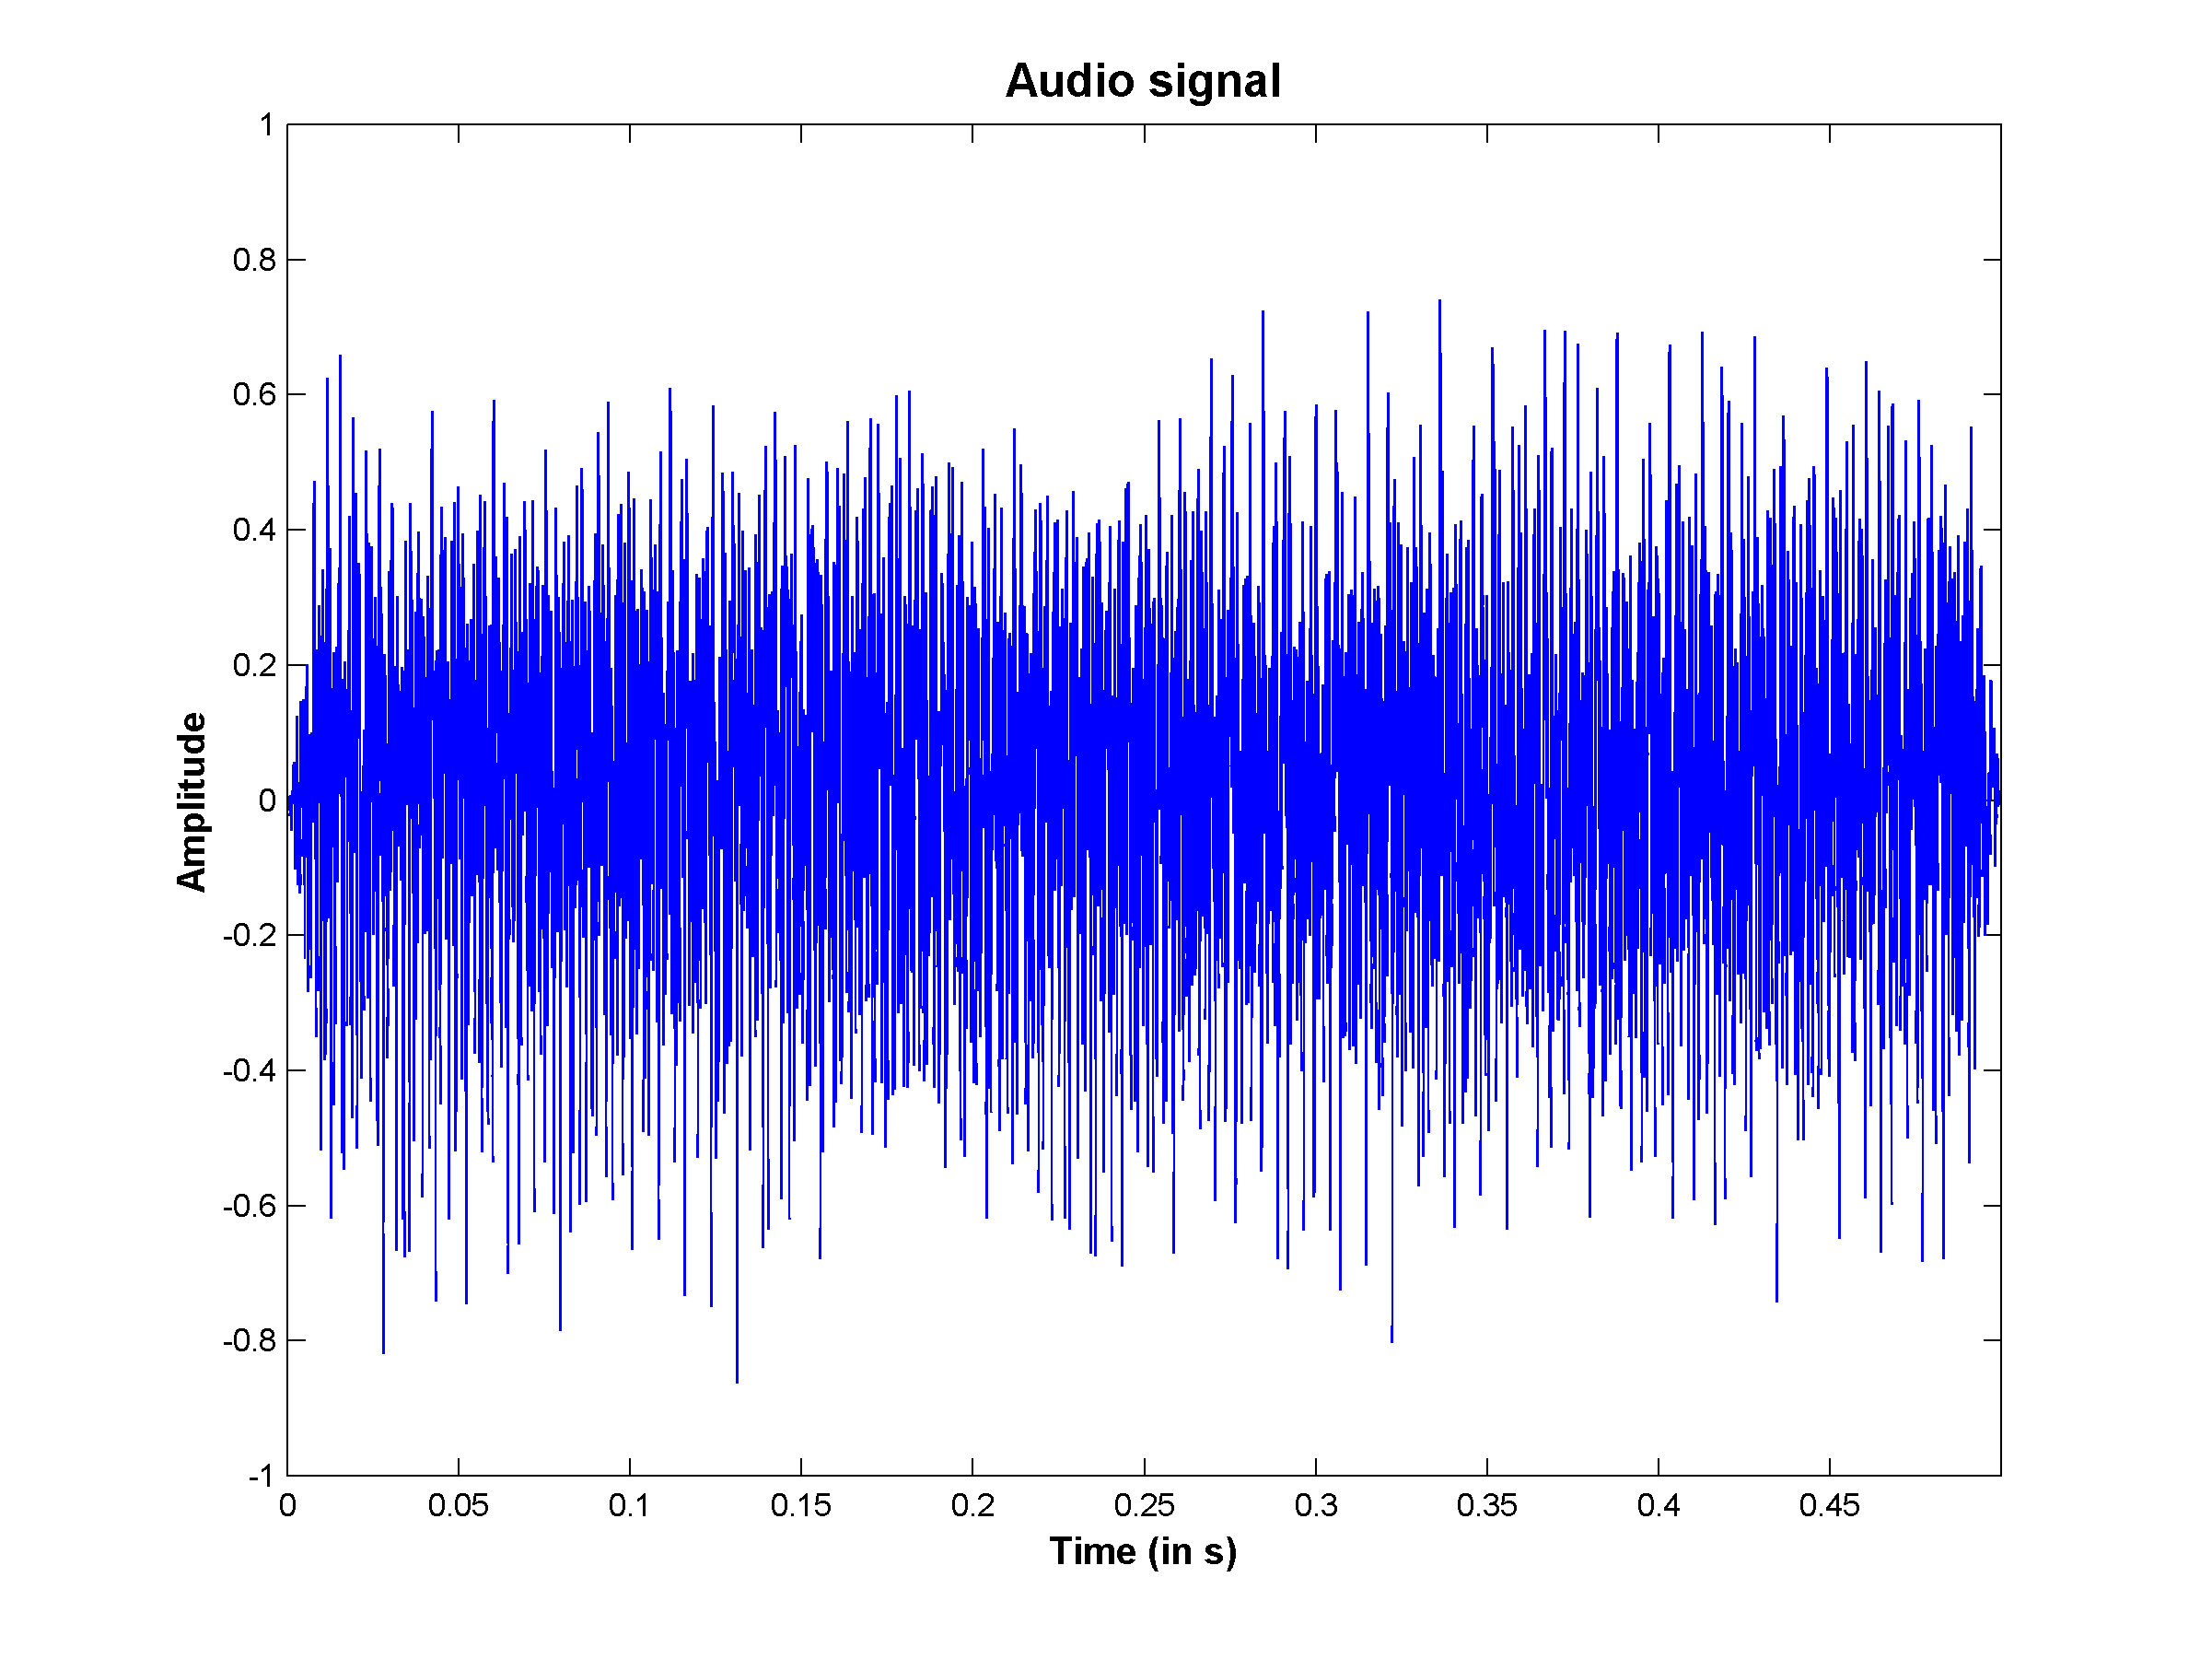
\includegraphics[width=\IPEMDefaultFigureWidth]{Graphics/ShepardCChordAudioSignal}
    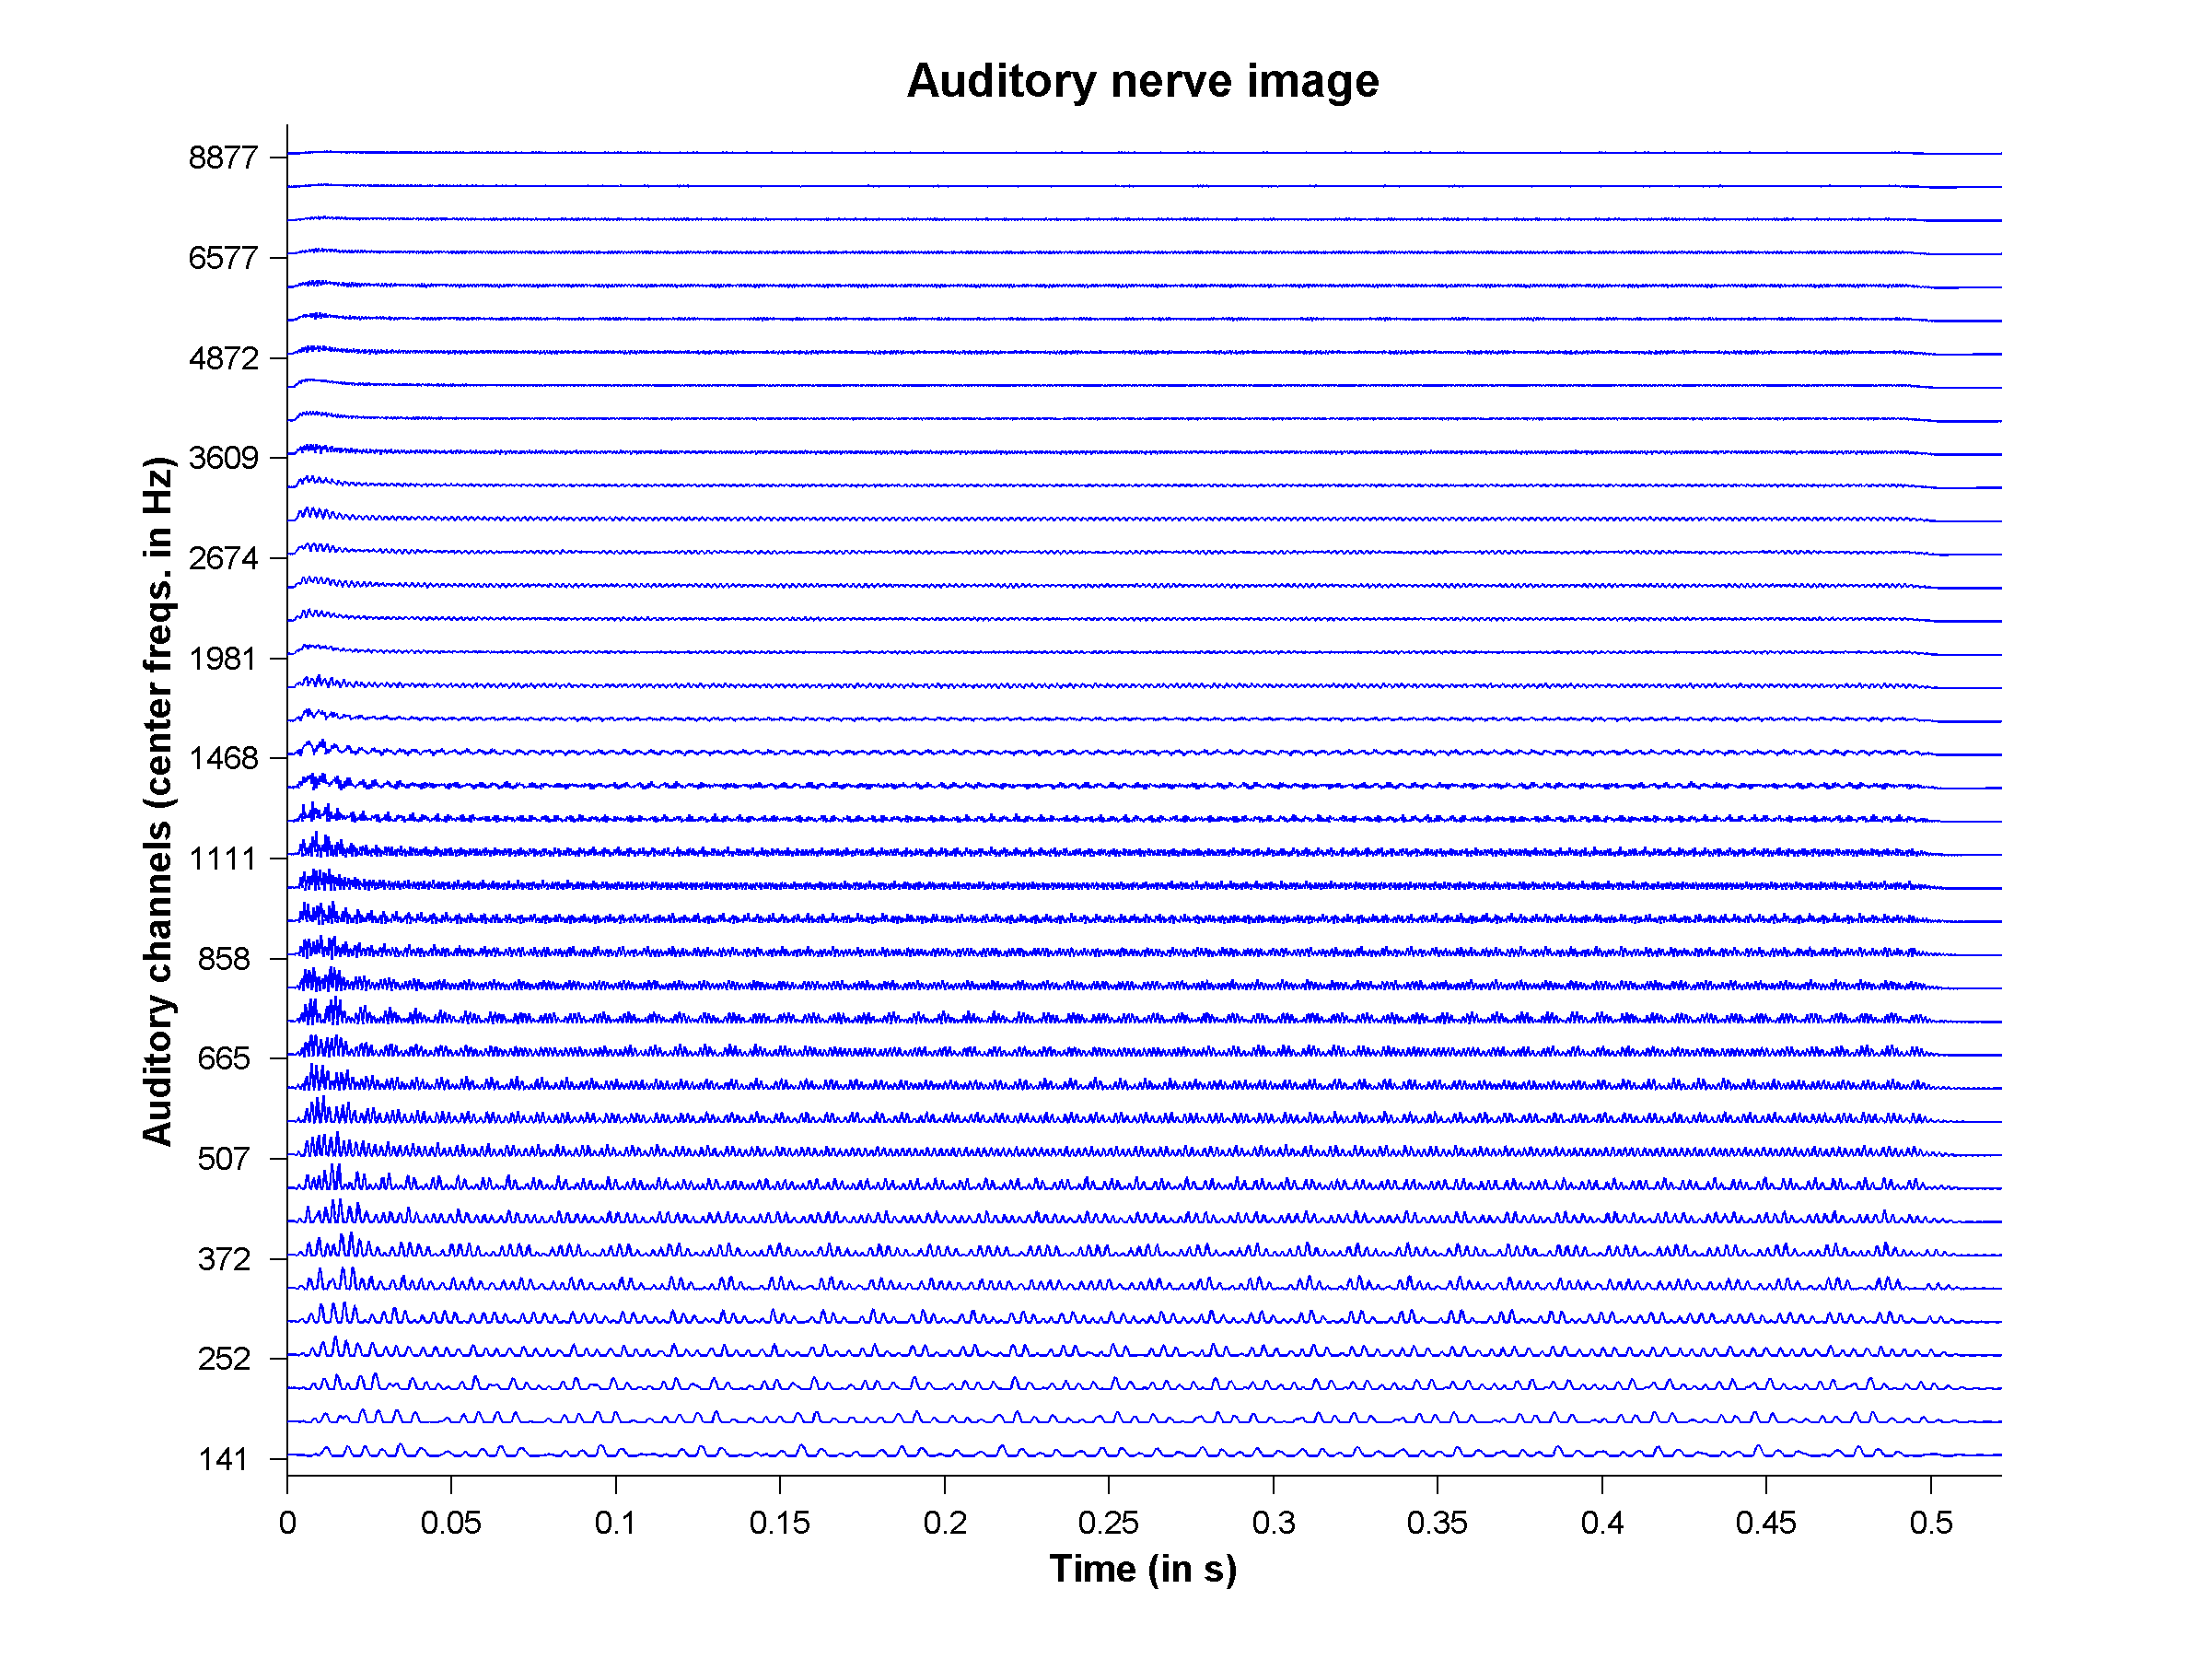
\includegraphics[width=\IPEMDefaultFigureWidth]{Graphics/ShepardCChordANI}
    \caption{Top: waveform of a C major chord using Shepard tones. Bottom: primary image}
    \label{Fig:ShepardCChordANIandAudioSignal}
\end{figure}
